\hypertarget{maggen_8cpp}{
\section{src/maggen.cpp File Reference}
\label{maggen_8cpp}\index{src/maggen.cpp@{src/maggen.cpp}}
}
Tool for Generation of Static Evaluators for Multi-plans Attribute Grammars.\par


{\tt \#include $<$stdio.h$>$}\par
{\tt \#include $<$iostream$>$}\par
{\tt \#include $<$fstream$>$}\par
{\tt \#include $<$string$>$}\par
{\tt \#include $<$time.h$>$}\par
{\tt \#include $<$sys/time.h$>$}\par
{\tt \#include $<$sys/stat.h$>$}\par
{\tt \#include $<$boost/tokenizer.hpp$>$}\par
{\tt \#include \char`\"{}../include/Maglib.h\char`\"{}}\par


Include dependency graph for maggen.cpp:\nopagebreak
\begin{figure}[H]
\begin{center}
\leavevmode
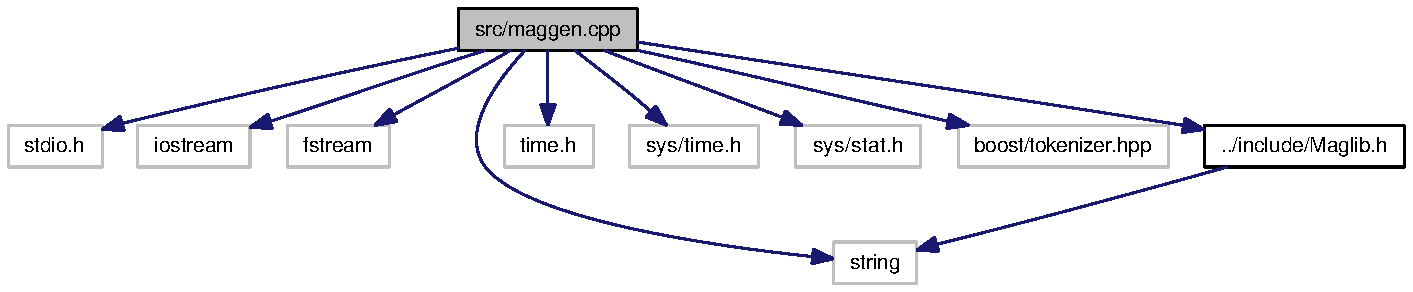
\includegraphics[width=357pt]{maggen_8cpp__incl}
\end{center}
\end{figure}
\subsection*{Namespaces}
\begin{CompactItemize}
\item 
namespace \hyperlink{namespacegenevalmag}{genevalmag}
\end{CompactItemize}
\subsection*{Functions}
\begin{CompactItemize}
\item 
const string \hyperlink{namespacegenevalmag_7bb640f537df129ffe4ed8cc5f703d90}{genevalmag::DEFAULT\_\-PATH} (\char`\"{}./out\_\-maggen/\char`\"{})
\item 
const string \hyperlink{namespacegenevalmag_a939bb88a9eee5dd79de6b2c0d9dc27b}{genevalmag::DEFAULT\_\-FILE\_\-NAME} (\char`\"{}mag\_\-eval\char`\"{})
\item 
const string \hyperlink{namespacegenevalmag_c01c19863afca7ad5f021857f24032c3}{genevalmag::DEFAULT\_\-INPUT\_\-FILE} (\char`\"{}/tmp/.input\_\-maggen\_\-default\char`\"{})
\item 
double \hyperlink{namespacegenevalmag_885d7859db4dd91f78bb7081be6ceacb}{genevalmag::timeval\_\-diff} (struct timeval $\ast$a, struct timeval $\ast$b)
\item 
bool \hyperlink{namespacegenevalmag_8d54caf5e5830cd48bf3265345928c3a}{genevalmag::check\_\-file\_\-exist} (const string \&strFilename)
\item 
bool \hyperlink{namespacegenevalmag_3bc888ab3b44c41a536427cf386f8c3d}{genevalmag::check\_\-name} (const string \&strFilename)
\item 
void \hyperlink{namespacegenevalmag_fe9d3ca44e4de7e9ebe9f47a62ed7aa5}{genevalmag::show\_\-help\_\-information} ()
\item 
bool \hyperlink{namespacegenevalmag_d3dcc8f1c112c2fee686c837e5250124}{genevalmag::parse\_\-parameters} (int argc, char $\ast$argv\mbox{[}$\,$\mbox{]}, string \&path\_\-input\_\-file, string \&path\_\-folder\_\-output, string \&name\_\-library, vector$<$ string $>$ \&headers)
\item 
int \hyperlink{maggen_8cpp_dedb285b02c41bde2158ded9cc9fd7ac}{main} (int argc, char $\ast$argv\mbox{[}$\,$\mbox{]}, char $\ast$envp\mbox{[}$\,$\mbox{]})
\end{CompactItemize}


\subsection{Detailed Description}
Tool for Generation of Static Evaluators for Multi-plans Attribute Grammars.\par
. 

\begin{Desc}
\item[Date:]09/02/2010 \end{Desc}
\begin{Desc}
\item[Author:]Kilmurray, Gerardo Luis $<$\href{mailto:gerakilmurray@gmail.com}{\tt gerakilmurray@gmail.com}$>$ 

Picco, Gonzalo Martín $<$\href{mailto:gonzalopicco@gmail.com}{\tt gonzalopicco@gmail.com}$>$ \end{Desc}


Definition in file \hyperlink{maggen_8cpp-source}{maggen.cpp}.

\subsection{Function Documentation}
\hypertarget{maggen_8cpp_dedb285b02c41bde2158ded9cc9fd7ac}{
\index{maggen.cpp@{maggen.cpp}!main@{main}}
\index{main@{main}!maggen.cpp@{maggen.cpp}}
\subsubsection[{main}]{\setlength{\rightskip}{0pt plus 5cm}int main (int {\em argc}, \/  char $\ast$ {\em argv}\mbox{[}$\,$\mbox{]}, \/  char $\ast$ {\em envp}\mbox{[}$\,$\mbox{]})}}
\label{maggen_8cpp_dedb285b02c41bde2158ded9cc9fd7ac}


Main method of the parsing. 

Definition at line 235 of file maggen.cpp.

References genevalmag::DEFAULT\_\-FILE\_\-NAME(), genevalmag::DEFAULT\_\-INPUT\_\-FILE(), genevalmag::DEFAULT\_\-PATH(), genevalmag::Maglib::gen\_\-evaluator(), genevalmag::parse\_\-parameters(), genevalmag::show\_\-help\_\-information(), and genevalmag::timeval\_\-diff().

Here is the call graph for this function:\nopagebreak
\begin{figure}[H]
\begin{center}
\leavevmode
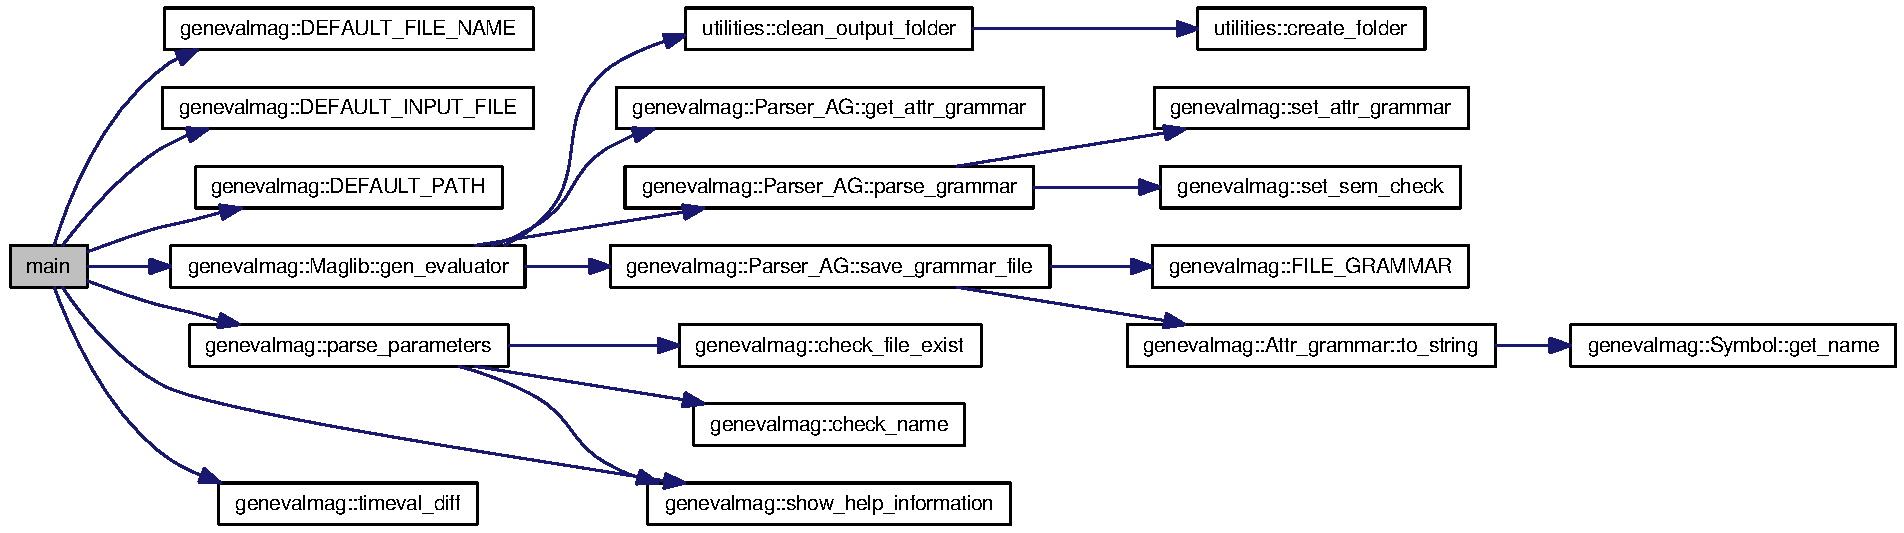
\includegraphics[width=420pt]{maggen_8cpp_dedb285b02c41bde2158ded9cc9fd7ac_cgraph}
\end{center}
\end{figure}
